%@author Brandon Roberts, Nate Olderman, Billy Rathje, DJ Maguddayao, Kyle Dybdal
%@date 9/23/13

\documentclass[12pt]{article}
\usepackage{graphicx}

\begin{document}

%-------------------------------------------------------------------------------------------------------------
% TITLE PAGE
%-------------------------------------------------------------------------------------------------------------

\begin{titlepage}
	\vspace*{\fill} %leave out given verticle space in a document
	\begin{center}
		{\Huge Story Creator Intermediate Report}\\ [0.5cm]	%make title huge and have .5cm space in between
		{\Large Brandon Roberts, Nate Olderman, Billy Rathje, DJ Maguddayao, Kyle Dybdal}\\[0.4cm]
		\today %put the date that the data is compiled
	\end{center}
	\vspace*{\fill}
\end{titlepage}

%------------------------------------------------------------------------------------------------------
%DESIGN SPECIFICATION
%----------------------------------------------------------------------------------------------------
\section{Design Specification}
	\subsection{Flow of Events}
	
The Story Creator module will be utilizing the Object Creator module, Visual Editor module, and the Animation modules work through the Sharing Framework.\\

The Sharing Framework will provide a database of the objects that were given to it by the Object Creators and a canvas to display the entire view.  These objects will be in the form of a .png and have a file that contains the methods and attributes that work for the particular object.  We will use the object .png itself to be placed on the story frame in order to display it to the storyteller.  To do this we will retrieve the information about the object from the Sharing Framework and then use the drawObject(...) method in order to display it on the frame.  Specifically we will be setting the original position where the object appears on the story panel.  \\


After the object is present on the story panel we will retrieve methods provided by the Visual Editor that were selected and edited by the storyteller.  We will then allow the storyteller to provide the parameters to these methods by the use of a drop down menu or by typing in the exact value (in the visual editor frame) they wish the method to use.  We will take the methods with parameters from the Visual Editor module and add the time that the user specified the action to occur.  The objects and their methods will be sent to the Animation module in a JSON format to interact with the objects at the specified time.  \\

\subsection{Interfaces and Code Flow}

\begin{verbatim}
Sharing Framework interface
---Object and Methods 
------Provided interface for VE (objects and the methods they have)
---------Visual Editor interface for changing the methods 
-------------Create Specific Object with time and parameters 
----------Interface to take master object and make JSON object 
-------------Animation to move specified object 
\end{verbatim}


The Story Creator module will implement an interface for the Sharing Framework in order retrieve objects and their methods.  This will be a required interface because the sharing framework will need to provide methods for downloading images and JSON representations of methods developed in the visual editor. The Story Creation Framework will need to request data from the server - not the other way around - so that is why the interface is a required interface.

The interface should include methods for downloading a .png by name, downloading methods for a .png by name, and getting the number of images and methods on the server.  \\

The Story Creator module will implement an interface for the Visual Editor module in order to retrieve the storyteller updated methods that may have changed from the original creation by the Animation module that was downloaded from the server with the object.  We will then attach the specific time and parameters provided by the storyteller to the unique object that is created by   the various components that the storyteller requires. \\ 



%Allow Visual Editor to specify the parameters possibly???


------Possibly drop down box of the objects methods when right click
------Possibly a class to retrieve information from Sharing and pass it around.

\subsection{Design Rational}
%Design Rationale-----------------------------
We chose to use this architecture so that we would be able to easily retrieve the objects from the Sharing Framework as well as the methods that the objects can use.  It will then be very simple to combine the objects taken from the Sharing Framework interface and combine it with the storyteller modified methods that the Visual Editor interface will provide.  
%----------------------------------------------

\subsection{Detailed formal spec}
\begin{itemize}
	\item Required Sharing Framework interface
	\item Required Visual Editor interface
	\item Provided Animation interface
\end{itemize}
\subsection{UML}

\subsection{Design interface}
The user interface will include a story panel which displays the story to the user and allows the user to interact with the objects displayed.  The Visual Editor will have a p


\subsection{Design details and restrictions}


%------------------------------------------------------------------------------------------------------
%PROJECT STATUS
%----------------------------------------------------------------------------------------------------
\section{Project Status}

\begin{figure}[ht!]
\centering
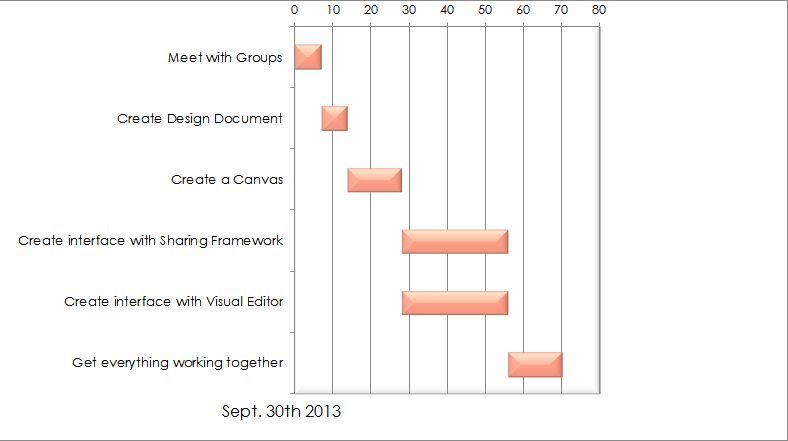
\includegraphics{GanttChart.png}
\caption{Gantt Chart}
\label{overflow}
\end{figure}

Nothing..........




%------------------------------------------------------------------------------------------------------
%
%----------------------------------------------------------------------------------------------------
\end{document}